
\documentclass[b5paper,9pt,twoside,openany]{article}

\usepackage{fontspec,xunicode,xltxtra}
\usepackage{listings}
\usepackage{color}
\usepackage{paralist}
\usepackage{qtree}
\usepackage{dirtree}
\usepackage{pstricks,pst-node}
\usepackage{tabularx}
\usepackage[a5paper]{geometry}
\usepackage[colorlinks=true,linkcolor=blue]{hyperref}


\XeTeXlinebreaklocale ``zh''
\XeTeXlinebreakskip = 0pt plus 1pt minus 0.1pt
\newfontfamily\song{SimSun}
\newfontfamily\hei{SimHei}
%\newfontfamily\kai{KaiTi}
%\newfontfamily\fsong{FangSong}
%\newfontfamily\nsong{NSimSun}
\newfontfamily\mshei{Microsoft YaHei}
\setmainfont{SimSun}

\begin{document}
\title{MM及初始化内存管理}
\section{启动}
Linux的内存模型规定内核态必须处于0xC000000以上的内存当中,而在系统启动阶段分页机制并未启动,这时候Linux的C程序的所有符号都处于这个界限之上,此时内核的C代码是没有办法直接运行的。因此vmlinux的起始部分代码只能通过汇编编写(在访问任意符号的时候,汇编语言可以通过读符号地址进行运算求得符号的物理而后进行操作)。这部分代码的主要工作就是初始化分页并启动分页机制,之后vmlinux就由物理内存的0x01000000处被映射在了虚拟地址的0xC1000000处,这时候所有代码都可以通过虚拟地址来访问符号了,C程序就可以正常工作了。
由于工作在物理内存上而gdb将vmlinux的符号表映射到物理内存,这部分代码的调试是比较麻烦的。接下来会介绍调试的步骤及代码分析,顺利通过这部分代码以后,内核将工作在虚拟内存地址上,gdb就可以实现代码级调试的了。

\section{启动调试}
在Linux启动时期并未启动分页机制,如果希望调试它必须使用gdb的硬件调试指令,比如设置断点使用hbreak命令。Linux启动之前加载程序会将它加载到物理内存0x01000000处。它的物理地址位于0x01000000处,也就是函数startup\_32的起始地址,它是vmlinux的入口地址。startup\_32是一个很长的函数,此处列出了部分重要部分的地址以方便用户设置断点。

\begin{tabular}{|c|c|c|c|}
\hline
作用  & 地址 & 结束地址 & 文件位置 \\
\hline
startup\_32 & 0x01000000 & 0x0100001d & kernel/head\_32.S:83 \\
\hline
清空bss段 & 0x0100001d & 0x01000031 & kernel/head\_32.S:103 \\
\hline
设置bootparam & 0x01000031 & 0x01000054 & kernel/head\_32.S:118 \\
\hline
x86子架构 & 0x01000054 & 0x01000077 & head\_32.S:145 \\
\hline
paging init & 0x0100007b & 0x010000cc & head\_32.S:174 \\
\hline
\end{tabular}

\subsection{x86子架构初始化}
在x86进入到保护模式之后,Linux会根据bootparam参数确定CPU类型并启动对应的初始代码。
\begin{lstlisting}
/* Paravirt-compatible boot parameters.  Look to see what architecture
 we're booting under. */
    movl pa(boot_params + BP_hardware_subarch), %eax
    cmpl $num_subarch_entries, %eax
    jae bad_subarch

    movl pa(subarch_entries)(,%eax,4), %eax
    subl $__PAGE_OFFSET, %eax
    jmp *%eax
bad_subarch:
    ud2
subarch_entries:
    .long default_entry             /* normal x86/PC */
    .long lguest_entry              /* lguest hypervisor */
    .long xen_entry                 /* Xen hypervisor */
    .long default_entry             /* Moorestown MID */
\end{lstlisting}
一般情况下,我们会进入到default\_entry继续运行。
\subsection{启动分页模式}
default\_entry的开始部分是分页模式的初始化,此处的代码按照两种模式实现(PAE模式及非PAE模式),PAE模式打开后能够访问64G物理内存。为了简化操作,我们需要将PAE关闭,在编译内核时大家可以查找"", 关闭它就好。
 
\lstset{language=[Motorola68k]Assembler, escapechar=@,style=gnuasmcode}
\begin{lstlisting}
page_pde_offset = (__PAGE_OFFSET >> 20);
    movl $pa(__brk_base), %edi
    movl $pa(swapper_pg_dir), %edx
    movl $PTE_IDENT_ATTR, %eax
10:
    leal PDE_IDENT_ATTR(%edi),%ecx          /* Create PDE entry */
    movl %ecx,(%edx)                        /* Store identity PDE entry */
    movl %ecx,page_pde_offset(%edx)         /* Store kernel PDE entry */
    addl $4,%edx
    movl $1024, %ecx
11:
    stosl
    addl $0x1000,%eax
    loop 11b
    /*
     * 是否覆盖到了结尾处, _end定义在vmlinux.lds.S,它是vmlinux末尾的地址
     */
    movl $pa(_end) + MAPPING_BEYOND_END + PTE_IDENT_ATTR, %ebp
    cmpl %ebp,%eax
    jb 10b
    addl $__PAGE_OFFSET, %edi
    movl %edi, pa(_brk_end)
    shrl $12, %eax
    movl %eax, pa(max_pfn_mapped)
    /* Do early initialization of the fixmap area */
    movl $pa(swapper_pg_fixmap)+PDE_IDENT_ATTR,%eax
    movl %eax,pa(swapper_pg_dir+0xffc)

    jmp  3f
\end{lstlisting}
有几个符号需要介绍一下, pa(physical address)是将虚拟地址转化为物理地址的一个宏,基本实现就是用符号的地址减去 PAGE\_OFFSET(这个值通常是0xC0000000).变量swapper\_pg\_dir用来保存PTE,而\_\_brk\_base用于保存PTE。
PDE\_IDENT\_ATTR是每个表项的属性值,GNUAS通过lea指令来计算。

\subsubsection{PTE的地址}
\_\_brk\_base是一个特殊的地址,这个地址的标识了vmlinux的尾部,也就是说在vmlinux在加入如内存之后,从\_\_brk\_base之后就没有vmlinux的数据和地址了,主部分内存是安全可用的。\_\_brk\_base只有在链接结束以后确定,所以它只能通过lds(ld script)来定义。以下代码节选自arch/x86/kernel/vmlinux.lds.S。
\begin{lstlisting}
. = ALIGN(PAGE_SIZE);
  .brk : AT(ADDR(.brk) - LOAD_OFFSET) {__brk_base = .;
  . += 64 * 1024;      /* 64k alignment slop space */
  *(.brk_reservation)  /* areas brk users have reserved */
  __brk_limit = .;
}
\end{lstlisting}

\subsubsection{覆盖地址}
\begin{lstlisting}
/*
 * This is how much memory in addition to the memory covered up to
 * and including _end we need mapped initially.
 * We need:
 *     (KERNEL_IMAGE_SIZE/4096) / 1024 pages (worst case, non PAE)
 *     (KERNEL_IMAGE_SIZE/4096) / 512 + 4 pages (worst case for PAE)
 *
 * Modulo rounding, each megabyte assigned here requires a kilobyte of
 * memory, which is currently unreclaimed.
 *
 * This should be a multiple of a page.
 *
 * KERNEL_IMAGE_SIZE should be greater than pa(_end)
 * and small than max_low_pfn, otherwise will waste some page table entries
 */

#if PTRS_PER_PMD > 1
#define PAGE_TABLE_SIZE(pages) (((pages) / PTRS_PER_PMD) + PTRS_PER_PGD)
#else
#define PAGE_TABLE_SIZE(pages) ((pages) / PTRS_PER_PGD)
#endif

/* Enough space to fit pagetables for the low memory linear map */
MAPPING_BEYOND_END = \
        PAGE_TABLE_SIZE(((1<<32) - __PAGE_OFFSET) >> PAGE_SHIFT) << PAGE_SHIFT
... 
    movl $pa(_end) + MAPPING_BEYOND_END + PTE_IDENT_ATTR, %ebp
    cmpl %ebp,%eax
    jb 10b
\end{lstlisting}
从上面的代码可以看到当初始化到某个值,页表就不再创建了,这个值就是page机制的覆盖范围,这个范围虽然是连续的,但却分成了两个部分,第一部分从0x00000000~0x00010000(物理内存的前1M),这里有许多用于特殊作用的内存,它们的虚拟地址与物理地址相同。第二部分就是内核内存了,在初始化阶段内核映射了1M~8M这个范围的内存到虚拟地址0xC1000000到0xC80000000上。

\subsubsection{初始化PTE}
PTE表项的内容保存在\%eax当中,它的初始值从0x0开始并带有属性PTE\_IDENT\_ATTR,它定义在文件arch/x86/include/asm/pgtable\_types.h当中。
\begin{lstlisting}
#define PTE_IDENT_ATTR   0x003          /* PRESENT+RW */
\end{lstlisting}

每一个PGD对应1024个PTE,通过stosl指令进行初始化,其中\%eax当中包含。
\begin{lstlisting}
    movl $PTE_IDENT_ATTR, %eax
10:
   /* 初始化 PGD */
   ...
    movl $1024, %ecx
11:
    stosl
    addl $0x1000,%eax
    loop 11b
\end{lstlisting}
上面的代码仅仅初始化了PTE项,大小保存存在\%ebp当中没初始化完成1024项都会比较一下以确定是否需要创建新的PTE项。

\subsubsection{常量}
x86架构下提供了两种分页机制,分别为两级和三级,对于i386 4G虚拟内存来说,采用了是两级地址映射,第一级叫做PGD(paging global dir),从第32位到第23位共10位,1024项,PTE(Page Table Entry)从第22位到第13位共10位,每一个PGD项包含1024个PTE项。这些常量定义在arch/x86/include/asm/pgtable-2level\_types.h(如果采用三级映射,那么常量定义在arch/x86/include/asm/pgtable-3level\_types.h)。
\begin{lstlisting}
#define PAGETABLE_LEVELS        2

#define PGDIR_SHIFT     22
#define PTRS_PER_PGD    1024

#define PTRS_PER_PTE    1024
\end{lstlisting}

\subsubsection{启动分页}
分页机制的启动需要三个步骤
\begin{itemize}
\item 设置PGD的入口地址到CR3
\item 设置CR0寄存器的PG位
\item 跳转至一下跳指令虚拟地址(否则将继续在当前地址运行,很有可能出错)
\end{itemize}
\begin{lstlisting}
/*
 * Enable paging
 */
    movl pa(initial_page_table), %eax
    movl %eax,%cr3          /* set the page table pointer.. */
    movl %cr0,%eax
    orl  $X86_CR0_PG,%eax
    movl %eax,%cr0          /* ..and set paging (PG) bit */
    ljmp $__BOOT_CS,$1f     /* Clear prefetch and normalize %eip */
\end{lstlisting}
在经过ljmp之后,系统进入到虚拟内存工作了,此时gdb已经可以将符号地址与虚拟地址相对应,调试时不需要再依赖于反汇编而可以进行源代码级调试了。这是一次飞跃,从此之后,调试程序进入一片坦途。
\section{e820}
\subsection{e820}
在实模式Linux通过e820获取到内存的分段信息,而后通过boot\_params传递给保护模式内核。在保护模式启动后,boot\_params的指针保存在寄存器\%esi当中,内核会将这段内存复制到保护模式下的boot\_params符号当中。
\subsection{e820}
\subsection{x86内存分布}
通过e820获取的内存布局信息在Linux系统当中会存放在/sys/firmware/memmap目录下,这些内存区域以目录的形式组织,可以通过一个简单的脚本来查看内存布局信息
\begin{lstlisting}[language=bash]
#!/bin/bash
 cd /sys/firmware/memmap
 for dir in * ; do
     start=$(cat $dir/start)
     end=$(cat $dir/end)
     type=$(cat $dir/type)
     printf ``%016x-%016x (%s)\n'' $start $[ $end +1] ``$type''
 done
\end{lstlisting}
它的输出如下
\begin{lstlisting}
0000000000000000-000000000009fc00 (System RAM)
000000000009fc00-00000000000a0000 (reserved)
00000000000f0000-0000000000100000 (reserved)
0000000000100000-000000007fff0000 (System RAM)
000000007fff0000-0000000080000000 (ACPI Tables)
00000000fffc0000-0000000100000000 (reserved)
\end{lstlisting}
\subsubsection{通过dmesg查看}
上面的map实际上是BISO初始化的分布,在系统初始化过程中对其中的一部分进行了修改,如图所示。

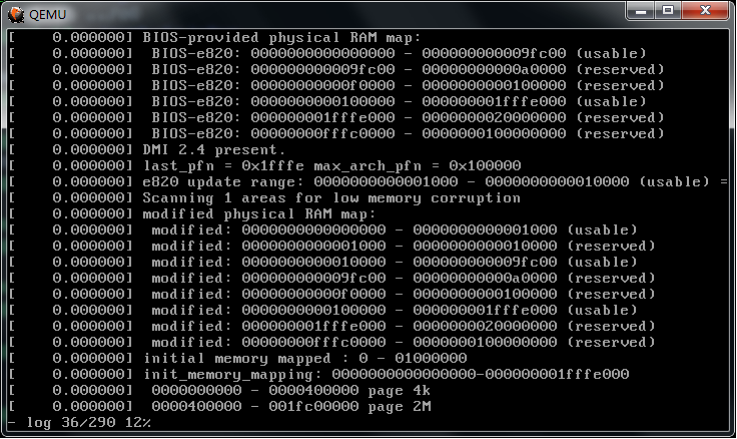
\includegraphics[scale=0.25]{images/e820}

\subsubsection{setup\_memory\_map}
在函数setup\_arch当中,setup\_memory\_map函数被调用,之后e820的memmap就做出了如图片当中的修改。它的内部调用了函数sanitize\_e820\_map,因为e820的某些memmap可能存在重叠,调用它的目的正是将这些重叠区域去掉。如果使用qemu来模拟机器是遇不到这种情况的。因此,我们直接避开他。


\subsection{通过early\_res分配内存}
e820仅仅保存了内存的布局信息,为了分配内存还需要做出进一步的努力以帮助系统记录那些内存被占用而那些内存仍可以被使用。在bootmem启动之前,承担这个责任的是early\_res,它与e820同样定义在文件arch/x86/kerenl/e820.c当中。结构体early\_res和它的一个全局数组early\_res便是记录内存分配信息的容器。
\begin{lstlisting}[language=C]
/*
 * Early reserved memory areas.
 */
#define MAX_EARLY_RES 20

struct early_res {
        u64 start, end;
        char name[16];
        char overlap_ok;
};
static struct early_res early_res[MAX_EARLY_RES] __initdata = {
        { 0, PAGE_SIZE, ``BIOS data page'' },     /* BIOS data page */
        {}
};
\end{lstlisting}
结构体当中overlap\_ok的意义比较复杂而且不算常用,暂且搁下后面介绍,结构器的其他字段意义比较明确也就不多说了。定义好了结构体之后,我们看看early\_res和e820如何配合分配内存。起到关键作用是函数find\_e820\_area和函数reserve\_early,其中函数find\_e820\_area的作用是寻找空闲区域而reserve\_early的作用是标记指定内存已经被分配。Linux当中包含很多这样的应用常见,例如下面的代码

\begin{lstlisting}[language=C]
// arch/x86/mm/init_32.c
void __init setup_bootmem_allocator(void) {
  bootmap_size = bootmem_bootmap_pages(max_low_pfn)<<PAGE_SHIFT;
  // find_e820_area从全局变量e820当中寻找一个能够容纳指定内存的段,且此段
  // 同时拥有足够的内存尚未被 reserve_early占用。
  // 而后使用reserve_early分配内存,实际上仅仅是在early_res数组当中增加一项
  // 告知内存已经被分配。
  bootmap = find_e820_area(0, max_pfn_mapped<<PAGE_SHIFT, bootmap_size,
                          PAGE_SIZE);
  reserve_early(bootmap, bootmap + bootmap_size, ``BOOTMAP'');
}
\end{lstlisting}
这段代码的作用是为bootmem的结构体分配空间。
\subsubsection{find\_e820\_area的实现}
\begin{algorithm}[H]
\SetAlgoLined
\BlankLine
\For{item in e820} {
  \If {item不是可分配内存或者空间不足} {
    continue;
  }
  \If {item当中未分配的内存已经不足} {
   continue;
  }
  返回内存地址
}
\BlankLine
返回空

\caption{find\_e820\_area}
\end{algorithm}

\subsection{与early\_res分配相关的函数}
\begin{itemize}
\item find\_overlapped\_early(u64 s, u64 e);
\item drop\_range(int i) 丢弃第i个slot
\item drop\_overlaps\_that\_are\_ok(u64 s, u64 e);
\item \_\_reserve\_early(u64 s, u64 e, char* name, int overlap)
\item reserve\_early\_overlap\_ok(u64 start, u64 end, char *name)
\end{itemize}

\subsection{overlap\_ok}

结构体early\_res的意义还是比较明确的,除了overlap\_ok,这个名字会让人误会以为它是“此区域可以覆盖更早的分配",但实际却不是这样,它的解释在函数reserve\_early\_overlap\_ok处。
\begin{lstlisting}[language=C]
/*
 * A few early reservtations come here.
 *
 * The 'overlap_ok' in the name of this routine does -not- mean it
 * is ok for these reservations to overlap an earlier reservation.
 * Rather it means that it is ok for subsequent reservations to
 * overlap this one.
 *
 * Use this entry point to reserve early ranges when you are doing
 * so out of "Paranoia", reserving perhaps more memory than you need,
 * just in case, and don't mind a subsequent overlapping reservation
 * that is known to be needed.
 *
 * The drop_overlaps_that_are_ok() call here isn't really needed.
 * It would be needed if we had two colliding 'overlap_ok'
 * reservations, so that the second such would not panic on the
 * overlap with the first.  We don't have any such as of this
 * writing, but might as well tolerate such if it happens in
 * the future.
 */
\end{lstlisting}

它的意思实际上是分配的内存可以在之后的分配时被overlap,即被使用。

\subsection{early\_res的应用场景}


\section{bootmem}
\subsection{为何需要bootmem}
bootmem的主要代码在mm/bootmem.c当中,从路径就可以看出bootmem已经是一个架构无关的内存管理框架了。

\subsection{bootmem框架}
bootmem使用bootmem\_data\_t来保存分配的内存,而且为了不再受到静态数组大小的限制,bootmem使用链表来记录分配的内存记录,这也是个巨大的飞跃。
\begin{lstlisting}[language=C]
// 文件 include/linux/bootmem.h
/*
 * node_bootmem_map is a map pointer - the bits represent all physical
 * memory pages (including holes) on the node.
 */
typedef struct bootmem_data {
  /* 当前节点负责管理的开始页帧及结束页帧 [node_min_pfn, node_low_pfn)
  unsigned long node_min_pfn;
  unsigned long node_low_pfn;
  
  /* 页帧使用情况的 bitmap */
  void *node_bootmem_map;
  unsigned long last_end_off;
  unsigned long hint_idx;
 
  /* 指向下一个节点 */
  struct list_head list;
} bootmem_data_t;

// 全局变量定义在 mm/bootmem.c 当中
bootmem_data_t bootmem_node_data[MAX_NUMNODES];
\end{lstlisting}

\subsubsection{bootmem初始化}
bootmem的初始化工作由init\_bootmem来完成,它通过调用init\_bootmem\_core来完成具体工作。
\begin{lstlisting}[language=C]
/**
 * init_bootmem - register boot memory
 * @start: pfn where the bitmap is to be placed
 * @pages: number of available physical pages
 *
 * Returns the number of bytes needed to hold the bitmap.
 */
unsigned long __init init_bootmem(unsigned long start, unsigned long pages)
{
  max_low_pfn = pages;
  min_low_pfn = start;

  /* NODE_DATA 访问的是 bootmem_node_data
   * 此处 bootmem 将由 start 开始的 pages 个页帧交给 bootmem 管理
   */
  return init_bootmem_core(NODE_DATA(0)->bdata, start, 0, pages);
}

static unsigned long __init init_bootmem_core(bootmem_data_t *bdata,
  unsigned long mapstart, unsigned long start, unsigned long end) {
  unsigned long mapsize;


  /* 此函数完成一些验证工作,并根据限制条件修改start和end的值 */
  mminit_validate_memmodel_limits(&start, &end);
  bdata->node_bootmem_map = phys_to_virt(PFN_PHYS(mapstart));
  bdata->node_min_pfn = start;
  bdata->node_low_pfn = end;

  /*
  * link_bootmem将bdata 放在合适的链表的位置上
  * 以保证链表是按照升序排列的
  */
  link_bootmem(bdata);

  /*
   * Initially all pages are reserved - setup_arch() has to
   * register free RAM areas explicitly.
   */
  mapsize = bootmap_bytes(end - start);
  memset(bdata->node_bootmem_map, 0xff, mapsize);

  return mapsize;
}

\end{lstlisting}

\subsection{分配内存}
分配内存的过程对于理解内存管理由为重要,bootmem提供了一组函数完成这些工作。首先来看页帧的分配和释放。
\subsubsection{page frame的分配和释放}
\begin{lstlisting}[language=C]
/* 此函数的功能是释放数据节点 bdata 的页帧
 * 范围是从 sidx 到 edix
 */
static void __init __free(bootmem_data_t *bdata,
                        unsigned long sidx, unsigned long eidx)
{
  unsigned long idx;
  if (bdata->hint_idx > sidx)
    bdata->hint_idx = sidx;

   /* 在 bitmap 上标记为可用 */
   for (idx = sidx; idx < eidx; idx++)
     if (!test_and_clear_bit(idx, bdata->node_bootmem_map))
       BUG();
}

/*
 * 分配从 sidx 到 edix 为止的页帧
 */
static int __init __reserve(bootmem_data_t *bdata, unsigned long sidx,
                        unsigned long eidx, int flags)
{
  unsigned long idx;
  int exclusive = flags & BOOTMEM_EXCLUSIVE;

  for (idx = sidx; idx < eidx; idx++)
    if (test_and_set_bit(idx, bdata->node_bootmem_map)) {
      if (exclusive) {
        __free(bdata, sidx, idx);
        return -EBUSY;
     }
  }
  return 0;
}

\end{lstlisting}
\subsubsection{bytes级别的分配与释放}
上面介绍了页帧的分配和释放,一般情况下,页帧最小也要4K,一般来说很少能一次用到这么多的内存,更多的情况还是以字节为单位分配的居多。
\begin{lstlisting}[language=C]
/**
 * __alloc_bootmem - allocate boot memory
 * @size: size of the request in bytes
 * @align: alignment of the region
 * @goal: preferred starting address of the region
 *
 * The goal is dropped if it can not be satisfied and the allocation will
 * fall back to memory below @goal.
 *
 * Allocation may happen on any node in the system.
 *
 * The function panics if the request can not be satisfied.
 */
void * __init __alloc_bootmem(unsigned long size, unsigned long align,
                              unsigned long goal)
{
  return ___alloc_bootmem(size, align, goal, 0);
}

static void * __init ___alloc_bootmem_nopanic(unsigned long size,
                                              unsigned long align,
                                              unsigned long goal,
                                              unsigned long limit)
{
  bootmem_data_t *bdata;
  void *region;

restart:
  region = alloc_arch_preferred_bootmem(NULL, size, align, goal, limit);
  if (region)
    return region;

  /* 对于 x86 来说, alloc_arch_preferred_bootmem 已经尝试了从
   * NODE_DATA(0) 处分配内存
   */
  list_for_each_entry(bdata, &bdata_list, list) {
    if (goal && bdata->node_low_pfn <= PFN_DOWN(goal))
      continue;
    if (limit && bdata->node_min_pfn >= PFN_DOWN(limit))
      break;

    region = alloc_bootmem_core(bdata, size, align, goal, limit);
    if (region)
      return region;
  }

  if (goal) {
    goal = 0;
    goto restart;
  }

  return NULL;
}

static void * __init alloc_arch_preferred_bootmem(bootmem_data_t *bdata,
                                                  unsigned long size,
                                                  unsigned long align,
                                                  unsigned long goal,
                                                  unsigned long limit) {
  if (WARN_ON_ONCE(slab_is_available()))
    return kzalloc(size, GFP_NOWAIT);

#ifdef CONFIG_HAVE_ARCH_BOOTMEM
  {
    bootmem_data_t *p_bdata;
    /* bootmem_arch_preferred_node 是一个宏,
     *  定义在 arch/x86/include/asm/mmzone_32.h 
     * 它返回 (NODE_DATA(0)->bdata) 
     */
    p_bdata = bootmem_arch_preferred_node(bdata, size, align,
                                          goal, limit);
    if (p_bdata)
      return alloc_bootmem_core(p_bdata, size, align,
                                goal, limit);
  }
#endif
  return NULL;
}


static void * __init alloc_bootmem_core(struct bootmem_data *bdata,
                                        unsigned long size, unsigned long align,
                                        unsigned long goal, unsigned long limit)
{
  unsigned long fallback = 0;
  unsigned long min, max, start, sidx, midx, step;

  if (!bdata->node_bootmem_map)
    return NULL;

  min = bdata->node_min_pfn;
  max = bdata->node_low_pfn;

  goal >>= PAGE_SHIFT;
  limit >>= PAGE_SHIFT;

  if (limit && max > limit)
    max = limit;
  if (max <= min)
    return NULL;

  /* 根据对其方式获取每次得到多少个页 */
  step = max(align >> PAGE_SHIFT, 1UL);

  if (goal && min < goal && goal < max)
    start = ALIGN(goal, step);
  else
    start = ALIGN(min, step);

  sidx = start - bdata->node_min_pfn;
  midx = max - bdata->node_min_pfn;

  if (bdata->hint_idx > sidx) {
    /*
     * Handle the valid case of sidx being zero and still
     * catch the fallback below.
     */
    fallback = sidx + 1;
    sidx = align_idx(bdata, bdata->hint_idx, step);
  }

  while (1) {
    int merge;
    void *region;
    unsigned long eidx, i, start_off, end_off;
 find_block:
    sidx = find_next_zero_bit(bdata->node_bootmem_map, midx, sidx);
    sidx = align_idx(bdata, sidx, step);
    eidx = sidx + PFN_UP(size);

    if (sidx >= midx || eidx > midx)
      break;

    for (i = sidx; i < eidx; i++)
      /* 测试接下来的几个 bit 是否处于可分配状态 */
      if (test_bit(i, bdata->node_bootmem_map)) {
        sidx = align_idx(bdata, i, step);
        if (sidx == i)
          sidx += step;
        goto find_block;
      }

    if (bdata->last_end_off & (PAGE_SIZE - 1) &&
        PFN_DOWN(bdata->last_end_off) + 1 == sidx)
      start_off = align_off(bdata, bdata->last_end_off, align);
    else
      start_off = PFN_PHYS(sidx);

    merge = PFN_DOWN(start_off) < sidx;
    end_off = start_off + size;

    bdata->last_end_off = end_off;
    bdata->hint_idx = PFN_UP(end_off);

    /* 分配内存,记录到 bitmap 上 */
    if (__reserve(bdata, PFN_DOWN(start_off) + merge,
                  PFN_UP(end_off), BOOTMEM_EXCLUSIVE))
      BUG();

    /* 将内存转化为虚拟内存 */
    region = phys_to_virt(PFN_PHYS(bdata->node_min_pfn) +
                          start_off);
    memset(region, 0, size);
    /*
     * The min_count is set to 0 so that bootmem allocated blocks
     * are never reported as leaks.
     */
    kmemleak_alloc(region, size, 0, 0);
    return region;
  }

  /* fallback 的作用 */
  if (fallback) {
    sidx = align_idx(bdata, fallback - 1, step);
    fallback = 0;
    goto find_block;
  }

  return NULL;
}

\end{lstlisting}

\subsection{early\_res到bootmem的转换}
在early\_res的工作完成以后,操作系统将内存管理的任务交给bootmem管理。转交过程中起到最大作用的是函数early\_res\_to\_bootmem,它将early\_res当中分配的内存转到bootmem的内存管理框架下。

\section{变量命名规则}
\begin{itemize}
\item pfn:  page frame num
\item va:   vitural address
\item pa:   physical address
\end{itemize}
\end{document}
